\section{Designing in Large-scale Socio-technical Systems}
\label{sec:design}
% Always give a unique label
% and use \ref{<label>} for cross-references
% and \cite{<label>} for bibliographic references
% use \sectionmark{}
% to alter or adjust the section heading in the running head


%\begin{figure}[h!]
%\begin{center}\footnotesize
%	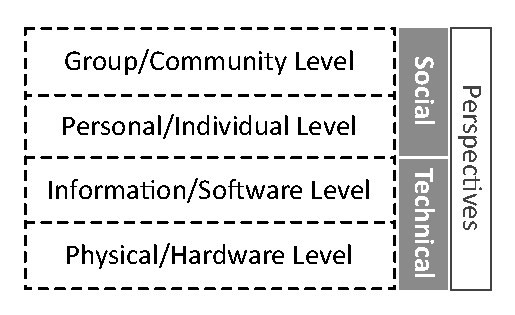
\includegraphics[width=1.0\linewidth]{img/sts_levels.pdf}\\
%	DSO (Distribution System Operators),  SSL (Secure Sockets Layer)
%	\caption{YouPower Platform Overview}\label{fig:platform}
%\end{center}
%\end{figure}

\begin{figure}[t]
\sidecaption[t]
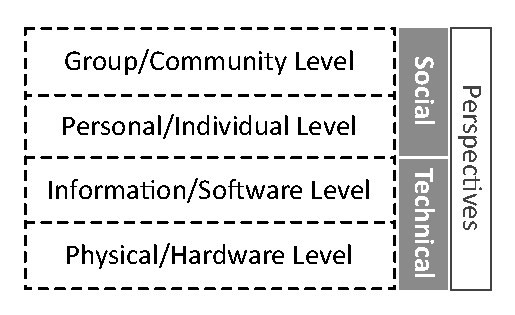
\includegraphics[scale=.68]{img/sts_levels.pdf}
\caption{Levels of socio-technical systems determined by different perspectives: the levels are not different systems but overlapping views of the  same system. Adapted from \cite{Whitworth2009,Whitworth2013}}
\label{fig:sts_levels} 
\end{figure}

The term ``socio-technical'' embodies both a research perspective and a subject matter \cite{Lee2001}. Facing a complex system, researchers from different disciplines often examine the system from their own perspectives. Engineers, for example, see hardware systems, computer scientists see information systems, psychologists see cognitive systems, sociologist see social systems -- in fact, no discipline has a monopoly on science and all those views are valid \cite{Whitworth2013}. 
The notion of system levels (shown in Fig.~\ref{fig:sts_levels}) illustrates this disciplinary isomorphism in socio-technical systems \cite{Whitworth2009,Whitworth2013}. Notably, the levels in Fig.~\ref{fig:sts_levels} are not different systems nor partitions of systems, but overlapping views of the same system corresponding to the engineering, computing, psychological and sociological perspectives \cite{Whitworth2009}. A socio-technical view is one that incorporates and interconnects all four levels of considerations: the upper two levels (Group/Community and Personal/Individual) together being social and the lower two (Information/Software and Physical/Hardware) technical. Each upper level can be seen as   ``arising'' or ``emerging'' from the lower levels. For example, personal cognitions ``emerge'' from neural information exchanges, which are supported by software that ``arises'' from hardware \cite{Whitworth2009}.
% 
The socio-technical systems view can be articulated as the recognition of three fundamental concepts as follows \cite{Sawyer2014}. 
%
%
\begin{description}
\item[\textit{First, the mutual constitution of people and technologies.}] 
This mutual constitution generates complex and dynamic interactions among technological capacities, social norms, histories, situated context, human choices, actions and so on. 
%
\item[\textit{Second, the contextual embeddedness of the mutuality.}] 
The context of a sociotechnical system is not taken as fixed or delineable. There are dynamic situational and temporal conditions that influence 
mutual adaptations throughout the course of design, development, deployment and uses of the system of interest. 
%
\item[\textit{Third, the importance of collective action.}] 
Collective action refers to the joint pursuit of one or more shared (potentially conflicting) goals by two or more interested parties such as problem owners, shareholders, users  and communities affected (without implying positive or negative outcomes). It shapes and is shaped by both the context and the technological components. 
\end{description}
%
%
Researchers who hold a socio-technical systems view investigate more than just the technological (sub-)system or just the social (sub-)system or even the two side by side, but also the phenomena that emerge when the two interact \cite{Lee2001}. A socio-technical approach tries to abstain from oversimplifications that seek a single or dominant cause of change, but studies the complexity, dynamic and uncertainty in the networks of institution, people and technological artefacts in the process of technologically involved change \cite{Sawyer2014}. 
%
Taking a socio-technical approach towards design has a number of implications for (i) the formulation of the design problem, (ii) the products of the design process, and (iii) the design process itself (BootCamp, BC?).

\begin{svgraybox}

Then the section proceeds with discussing the three implications (1) making relation to the three fundamental concepts (2) using the literature mentioned (can be expanded) in the next grey box 

\runinhead{Understanding and formulation of the design problem or situation}

The understanding and formulation of the design problem 

 It is not straightforward what needs to be taken into consideration in relation to the design. What systems boundaries to choose. the question of systems boundaries is an issue for technical systems and even becomes more difficult for social technical systems
what are the issues to be addressed.[BC]

Ill-structured problem

\runinhead{Products of the design process} these not only consists of technological artifacts but also may include rules for behaviour, policies, etc. through which the designer wish to intervene in social-technical systems. what is it that we are designing? 

\runinhead{Design process} The design process can be seen as a decision-making process where the problem owners, shareholders, users, etc. participate to represent their interests. It is often conceived and implemented in participatory decision-making processes actively involving stakeholders

Large-scale socio-technical systems are often not designed as a whole but incrementally ``piece by piece'' evolving from legacy systems (BC). Designers are therefore working \textit{in} the context of some socio-technical system with the intention of changing or improving some part of that system [BC]. This means that what matters more in the design is the design process itself, more than the ``final status'' of the system \cite{Shin2014, need more ref} because the socio-technical system keeps evolving and exhibits emergent behaviour \cite{Nikolic2009}. An important  goal of the design process is to make the design (a product or system) relevant to the evolving context \cite{Shin2014, need more ref} as social and technical artifacts exist within their socio-technical context [BC]. 

\end{svgraybox}



\begin{svgraybox}
can be put in the discussion: 
acontextual and detemporalized perspective approaches , general solution ., is self-limiting 
focus on situating work and seek to examine all contextual factors , this types of inquiry attempt to construct a holistic view of context: one that does not diminish or remove contextual elements, even those with limited influence. 
paying little attention to the environment of the organization and temporal dimension of technological innovation  \cite{Sawyer2014}
\end{svgraybox}


\begin{svgraybox}
Use and combine content in: (the literature can be connected, e.g. problems mentioned in Norman and Baxter  can be mapped to the four layers in Whitworth )
\begin{enumerate}
\item \cite{Norman2015} (design problems in large-scale socio-technical systems) and 
\item \cite{Baxter2011} (socio-technical approach to systems engineering)
\item \cite{Whitworth2009} (four system levels of Socio-tehnical systems); 
\item \cite{Shin2014} (a very good article about IoT, socio-technical perspective )
\item see also https://medium.com/rettigs-notes/notes-on-sociotechnical-systems-design-178f161bc9e8 
\end{enumerate}
\end{svgraybox}

